\documentclass[12pt]{article}

% --------------------------------------------------------
% CLASSIC LATEX FONTS/ENCODING
% --------------------------------------------------------
\usepackage[T1]{fontenc}
\usepackage[utf8]{inputenc}
\usepackage{lmodern} % loads Latin Modern fonts in a standard way

% --------------------------------------------------------
% PAGE & FONT SETUP
% --------------------------------------------------------
\usepackage[margin=1in]{geometry}
\usepackage{ragged2e}
\usepackage{graphicx}
\usepackage{float}
\usepackage{hyperref}
\hypersetup{%
  colorlinks=true,
  linkcolor=blue!50!black,
  urlcolor=blue!50!black
}

\setlength{\parskip}{6pt}
\setlength{\parindent}{0pt}

% --------------------------------------------------------
% COLOR & SECTION STYLING
% --------------------------------------------------------
\usepackage{xcolor}
\usepackage{sectsty}
\usepackage{titlesec}

\definecolor{mainDark}{HTML}{2C3E50}
\definecolor{mainLight}{HTML}{ECF0F1}
\definecolor{accentColor}{HTML}{3498DB}
\definecolor{boxBg}{HTML}{F8F9FA}

\sectionfont{\color{mainDark}\huge}
\subsectionfont{\color{mainDark}\Large}
\subsubsectionfont{\color{mainDark}\large}

\titlespacing*{\section}{0pt}{0.8em}{0.6em}
\titlespacing*{\subsection}{0pt}{0.7em}{0.4em}

% --------------------------------------------------------
% CODE LISTINGS (MINTED)
% --------------------------------------------------------
\usepackage{minted}
\usemintedstyle{friendly}

% --------------------------------------------------------
% TIKZ FOR DIAGRAMS
% --------------------------------------------------------
\usepackage{tikz}
\usetikzlibrary{shapes,arrows,positioning,calc,arrows.meta,shapes.misc}

% Custom styles for boxes/arrows
\tikzset{%
  serviceBox/.style={%
    rectangle,
    rounded corners,
    draw=mainDark,
    fill=boxBg,
    text width=3.2cm,
    minimum height=1.2cm,
    align=center
  },
  arrowLine/.style={%
    -{Latex[length=3mm,width=2mm]},
    thick,
    color=mainDark
  },
  cloudService/.style={%
    cloud,
    draw=mainDark,
    fill=boxBg,
    cloud puffs=15,
    cloud puff arc=120,
    aspect=2,
    minimum width=2.6cm,
    align=center
  },
  database/.style={%
    cylinder,
    cylinder uses custom fill,
    cylinder body fill=boxBg,
    cylinder end fill=boxBg,
    draw=mainDark,
    shape aspect=0.7,
    minimum height=2.2cm,
    minimum width=1.4cm,
    align=center
  },
  userFigure/.style={%
    rectangle,
    rounded corners,
    draw=mainDark,
    fill=green!15,
    text width=2.7cm,
    minimum height=1.1cm,
    align=center
  }
}

% --------------------------------------------------------
% TITLE
% --------------------------------------------------------
\title{%
  \vspace{-2cm}
  \textbf{\color{mainDark}\Huge A Modern, Visual Introduction to AWS}\\
  \vspace{0.2cm}
  \large \textit{(Beginner-Friendly Edition)}
}
\author{}
\date{}

\begin{document}
\maketitle
\vspace{-1cm}

% --------------------------------------------------------
% INTRO
% --------------------------------------------------------
\section*{Introduction}
\addcontentsline{toc}{section}{Introduction}
\justifying

\textbf{Amazon Web Services (AWS)} is a platform where you can rent computing resources---like virtual machines or storage---on demand. Traditionally, you'd buy your own physical servers and handle hardware yourself, but AWS eliminates much of that work, letting you pay only for the services you use.

\begin{center}
    \resizebox{0.9\textwidth}{!}{%
        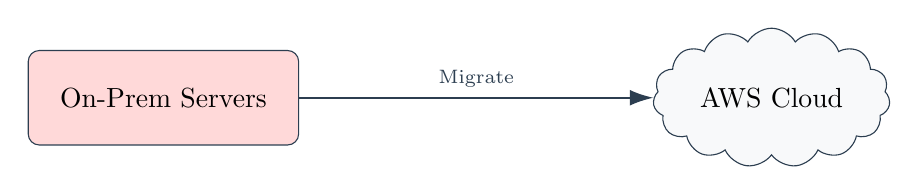
\begin{tikzpicture}[node distance=3cm]
            \node[serviceBox, fill=red!15, text width=3.2cm] (onprem) {On-Prem Servers};
            \node[cloudService, right=4.5cm of onprem] (awsCloud) {AWS Cloud};
            \draw[arrowLine] (onprem) -- node[above]{\scriptsize Migrate} (awsCloud);
        \end{tikzpicture}
    }
\end{center}

Instead of maintaining a data center, AWS handles physical security, power, cooling, and more. This gives you more time to build solutions rather than worry about hardware.

\begin{itemize}
    \item Learn how AWS compares to traditional (on-premises) servers.
    \item Explore the major AWS services and how they fit together.
    \item See diagrams that illustrate common AWS architectures.
    \item Check out simple project ideas to get hands-on experience.
\end{itemize}

Let's begin!

\clearpage

% --------------------------------------------------------
% 1. COMPARING ON-PREMISES VS. AWS
% --------------------------------------------------------
\section{Comparing On-Premises vs. AWS}
\justifying

\subsection{High-Level Differences}

\begin{center}
    \resizebox{0.95\textwidth}{!}{%
        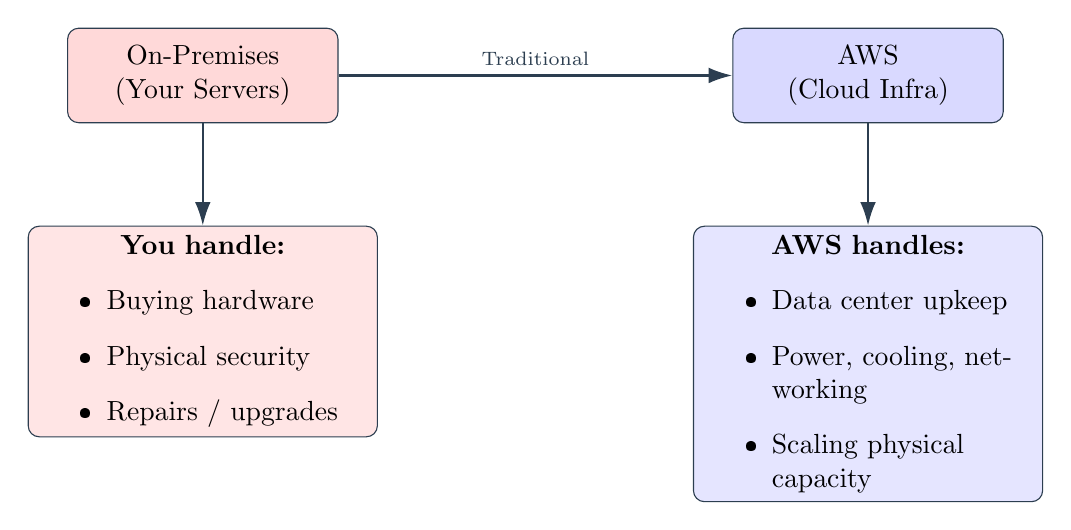
\begin{tikzpicture}[node distance=2.7cm]
            \node[serviceBox, text width=3.2cm, fill=red!15] (onprem) {On-Premises\\(Your Servers)};
            \node[serviceBox, text width=3.2cm, fill=blue!15, right=5cm of onprem] (cloud) {AWS\\(Cloud Infra)};

            \draw[arrowLine] (onprem) -- node[above]{\scriptsize Traditional} (cloud);

            \node[serviceBox, fill=red!10, below=1.3cm of onprem, text width=4.2cm] (onpremDetails)
            {\textbf{You handle:}
                \begin{itemize}
                    \item Buying hardware
                    \item Physical security
                    \item Repairs / upgrades
                \end{itemize}
            };
            \node[serviceBox, fill=blue!10, below=1.3cm of cloud, text width=4.2cm] (cloudDetails)
            {\textbf{AWS handles:}
                \begin{itemize}
                    \item Data center upkeep
                    \item Power, cooling, networking
                    \item Scaling physical capacity
                \end{itemize}
            };

            \draw[arrowLine] (onprem) -- (onpremDetails);
            \draw[arrowLine] (cloud) -- (cloudDetails);

        \end{tikzpicture}
    }
\end{center}

On-premises means you manage everything yourself: building or renting space for servers, dealing with hardware failures, etc. AWS handles those tasks and charges you for the resources you actually use.

\clearpage

% --------------------------------------------------------
% 2. WHAT IS AWS?
% --------------------------------------------------------
\section{What is AWS?}
\justifying

\subsection{Core Service Areas}
AWS offers many types of services, but some core ones include:
\begin{itemize}
    \item \textbf{Compute (EC2, Lambda)}: How you run your code or applications.
    \item \textbf{Storage (S3, EBS)}: Where you store files, backups, or disk volumes.
    \item \textbf{Databases (RDS, DynamoDB)}: Choose relational (SQL) or NoSQL data stores.
    \item \textbf{Networking (VPC, CloudFront)}: Control network traffic and deliver content globally.
    \item \textbf{Analytics (Kinesis, Athena)}: Process data streams or query large data sets.
    \item \textbf{Machine Learning (SageMaker)}: Tools to build and train models, then deploy them.
\end{itemize}

\subsection{Regions and Availability Zones}
AWS organizes its data centers worldwide into \textbf{Regions} (like US East 1, EU West 1, etc.). Each Region has multiple \textbf{Availability Zones} to improve reliability and fault tolerance.

\begin{center}
    \resizebox{0.95\textwidth}{!}{%
        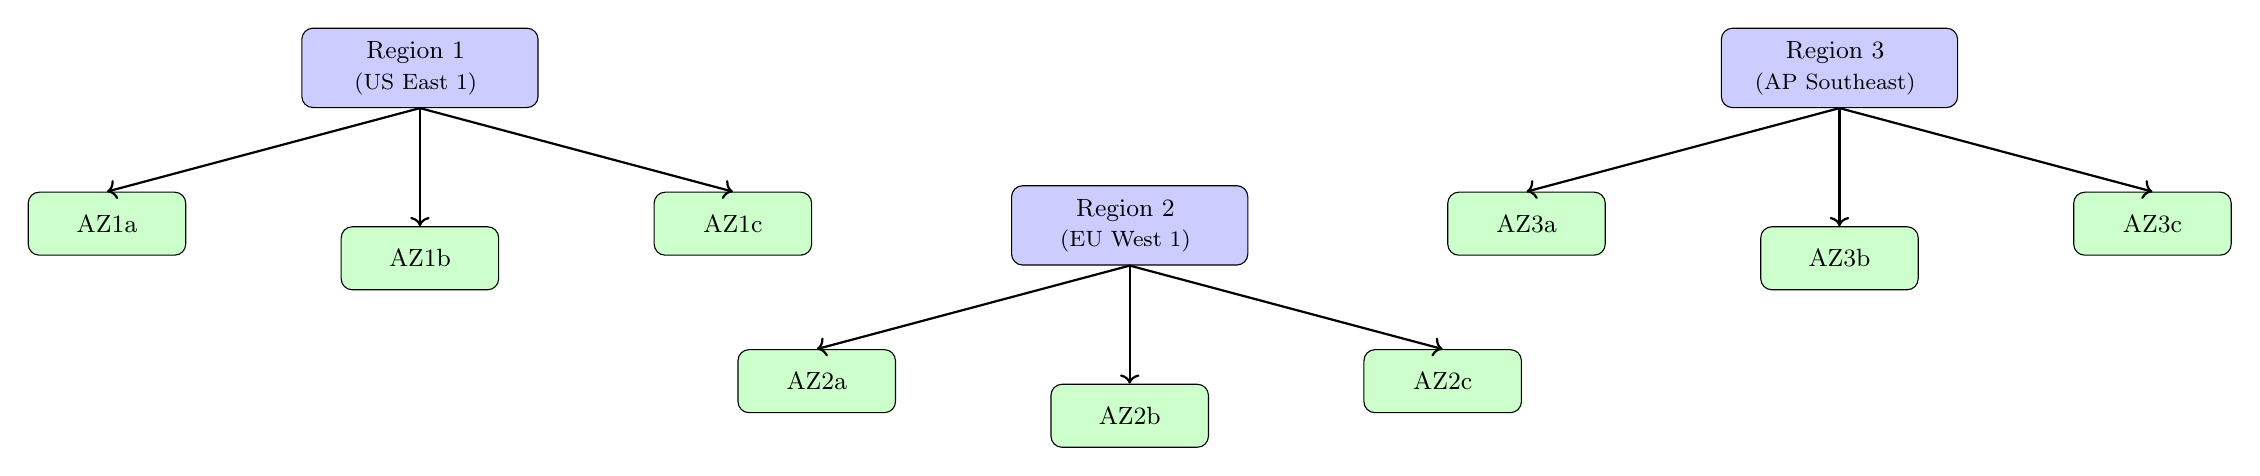
\begin{tikzpicture}[node distance=1.5cm]
            % Styles for region boxes
            \tikzset{%
                regionStyle/.style={%
                        rectangle,
                        rounded corners,
                        draw=black,
                        text centered,
                        fill=blue!20,
                        minimum width=3cm,
                        minimum height=1cm,
                        font=\small,
                        align=center
                    },
                azStyle/.style={%
                        rectangle,
                        rounded corners,
                        draw=black,
                        fill=green!20,
                        text centered,
                        minimum width=2cm,
                        minimum height=0.8cm,
                        font=\small
                    },
                arrowLine/.style={%
                        ->,
                        thick
                    }
            }

            % Region 1 with three AZs
            \node[regionStyle] (region1) {%
                \begin{tabular}{c}
                    Region 1 \\
                    {\footnotesize (US East 1)}
                \end{tabular}
            };

            \node[azStyle, below left=of region1, xshift=-0.4cm] (az1a) {AZ1a};
            \node[azStyle, below=of region1] (az1b) {AZ1b};
            \node[azStyle, below right=of region1, xshift=0.4cm] (az1c) {AZ1c};

            \draw[arrowLine] (region1.south) -- (az1a.north);
            \draw[arrowLine] (region1.south) -- (az1b.north);
            \draw[arrowLine] (region1.south) -- (az1c.north);

            % Region 2 with three AZs
            \node[regionStyle, right=6cm of region1, yshift=-2cm] (region2) {%
                \begin{tabular}{c}
                    Region 2 \\
                    {\footnotesize (EU West 1)}
                \end{tabular}
            };

            \node[azStyle, below left=of region2, xshift=-0.4cm] (az2a) {AZ2a};
            \node[azStyle, below=of region2] (az2b) {AZ2b};
            \node[azStyle, below right=of region2, xshift=0.4cm] (az2c) {AZ2c};

            \draw[arrowLine] (region2.south) -- (az2a.north);
            \draw[arrowLine] (region2.south) -- (az2b.north);
            \draw[arrowLine] (region2.south) -- (az2c.north);

            % Region 3 with three AZs
            \node[regionStyle, right=6cm of region2, yshift=+2cm] (region3) {%
                \begin{tabular}{c}
                    Region 3 \\
                    {\footnotesize (AP Southeast)}
                \end{tabular}
            };

            \node[azStyle, below left=of region3, xshift=-0.4cm] (az3a) {AZ3a};
            \node[azStyle, below=of region3] (az3b) {AZ3b};
            \node[azStyle, below right=of region3, xshift=0.4cm] (az3c) {AZ3c};

            \draw[arrowLine] (region3.south) -- (az3a.north);
            \draw[arrowLine] (region3.south) -- (az3b.north);
            \draw[arrowLine] (region3.south) -- (az3c.north);
        \end{tikzpicture}
    }
\end{center}

\clearpage

% --------------------------------------------------------
% 3. HOW COMPANIES USE AWS
% --------------------------------------------------------
\section{How Companies Use AWS}
\justifying

\subsection{Hosting Websites}
From a simple static site stored in \textbf{S3} to a large dynamic application running on \textbf{EC2} or container services.

\begin{center}
    \resizebox{0.92\textwidth}{!}{%
        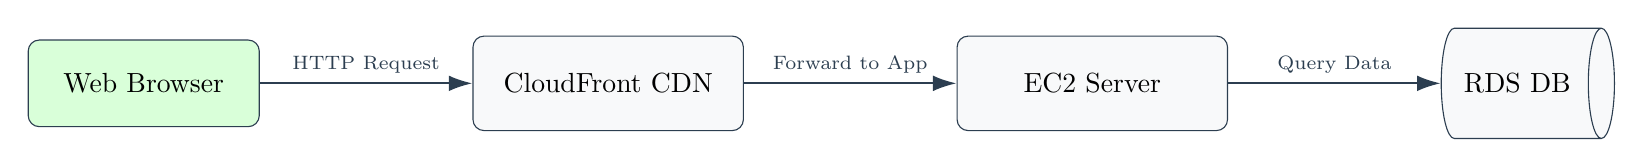
\begin{tikzpicture}[node distance=2.7cm]
            \node[userFigure] (user) {Web Browser};
            \node[serviceBox, right=2.7cm of user] (cloudfront) {CloudFront CDN};
            \node[serviceBox, right=2.7cm of cloudfront] (ec2) {EC2 Server};
            \node[database, right=2.7cm of ec2] (rds) {RDS DB};

            \draw[arrowLine] (user) -- node[above]{\scriptsize HTTP Request} (cloudfront);
            \draw[arrowLine] (cloudfront) -- node[above]{\scriptsize Forward to App} (ec2);
            \draw[arrowLine] (ec2) -- node[above]{\scriptsize Query Data} (rds);
        \end{tikzpicture}
    }
\end{center}

\subsection{Data Storage and Backup}
Companies keep backups, media, or data archives in \textbf{S3}, which provides high durability and easy retrieval.

\subsection{Application Development}
Developers build microservices using \textbf{Lambda} and \textbf{API Gateway}, then store structured data in \textbf{RDS} or \textbf{DynamoDB}.

\clearpage

% --------------------------------------------------------
% 4. SIMPLE AWS ARCHITECTURES
% --------------------------------------------------------
\section{Simple AWS Architectures}
\justifying

Below are more small diagrams that explain common patterns.

\subsection{Serverless File Processor}
\begin{center}
    \resizebox{\textwidth}{!}{%
        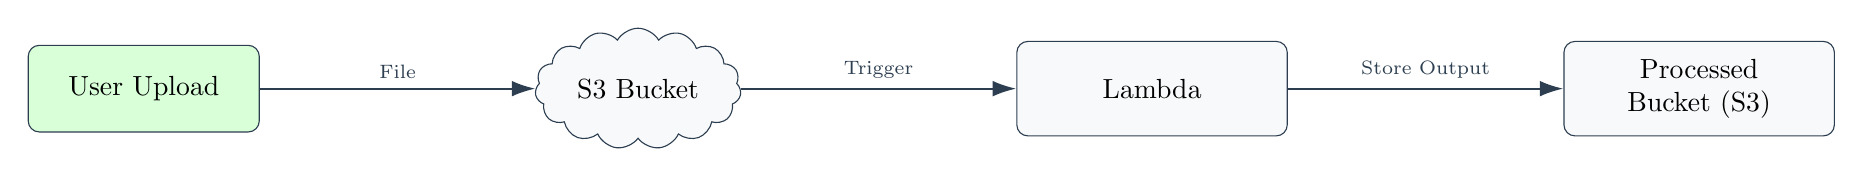
\begin{tikzpicture}[node distance=3cm]
            \node[userFigure] (upload) {User Upload};
            \node[cloudService, right=3.5cm of upload] (s3) {S3 Bucket};
            \node[serviceBox, right=3.5cm of s3] (lambda) {Lambda};
            \node[serviceBox, right=3.5cm of lambda] (done) {Processed Bucket (S3)};

            \draw[arrowLine] (upload) -- node[above]{\scriptsize File} (s3);
            \draw[arrowLine] (s3) -- node[above]{\scriptsize Trigger} (lambda);
            \draw[arrowLine] (lambda) -- node[above]{\scriptsize Store Output} (done);
        \end{tikzpicture}
    }
\end{center}

\subsection{Event-Driven Workflow}
\begin{center}
    \resizebox{0.9\textwidth}{!}{%
        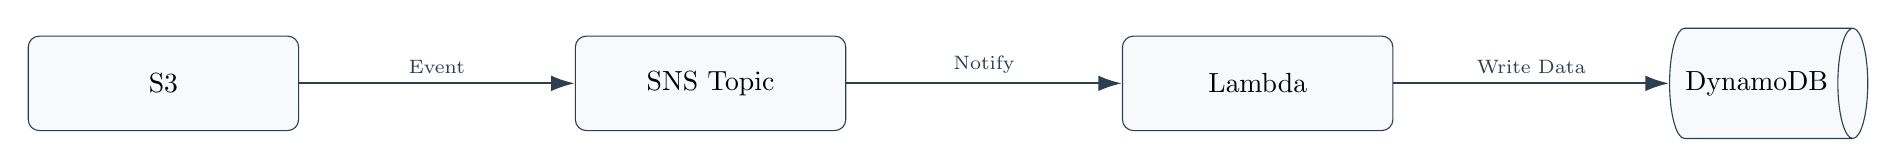
\begin{tikzpicture}[node distance=3cm]
            \node[serviceBox] (s3) {S3};
            \node[serviceBox, right=3.5cm of s3] (sns) {SNS Topic};
            \node[serviceBox, right=3.5cm of sns] (lambda) {Lambda};
            \node[database, right=3.5cm of lambda] (ddb) {DynamoDB};

            \draw[arrowLine] (s3) -- node[above]{\scriptsize Event} (sns);
            \draw[arrowLine] (sns) -- node[above]{\scriptsize Notify} (lambda);
            \draw[arrowLine] (lambda) -- node[above]{\scriptsize Write Data} (ddb);
        \end{tikzpicture}
    }
\end{center}

\subsection{Monitoring with CloudWatch}
\begin{center}
    \resizebox{0.85\textwidth}{!}{%
        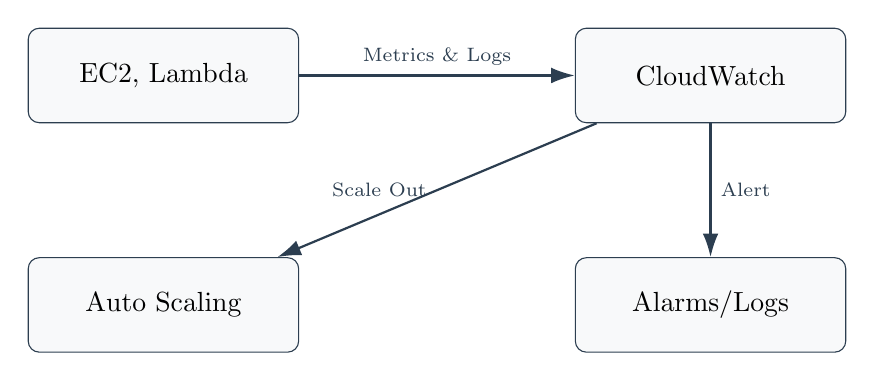
\begin{tikzpicture}[node distance=3cm]
            \node[serviceBox] (resource) {EC2, Lambda};
            \node[serviceBox, right=3.5cm of resource] (cw) {CloudWatch};
            \node[serviceBox, below=1.7cm of cw] (alarms) {Alarms/Logs};
            \node[serviceBox, below=1.7cm of resource] (autoscale) {Auto Scaling};

            % Fixed this line by escaping the ampersand:
            \draw[arrowLine] (resource) -- node[above]{\scriptsize Metrics \& Logs} (cw);
            \draw[arrowLine] (cw) -- node[right]{\scriptsize Alert} (alarms);
            \draw[arrowLine] (cw) -- node[left]{\scriptsize Scale Out} (autoscale);
        \end{tikzpicture}
    }
\end{center}

\clearpage

% --------------------------------------------------------
% 5. KEY AWS SERVICES (SIMPLIFIED)
% --------------------------------------------------------
\section{Key AWS Services (Simplified)}
\justifying

\subsection{S3 vs. EBS (Two Types of Storage)}
\begin{center}
    \resizebox{0.85\textwidth}{!}{%
        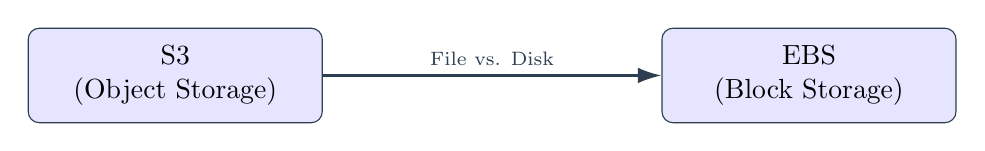
\begin{tikzpicture}[node distance=4.3cm]
            \node[serviceBox, fill=blue!10, text width=3.5cm] (s3) {S3\\(Object Storage)};
            \node[serviceBox, fill=blue!10, text width=3.5cm, right=4.3cm of s3] (ebs) {EBS\\(Block Storage)};

            \draw[arrowLine] (s3) -- node[above]{\scriptsize File vs. Disk} (ebs);
        \end{tikzpicture}
    }
\end{center}
\textbf{S3} is for storing files ("objects") in buckets. \textbf{EBS} acts like a hard drive attached to an EC2 server.

\subsection{EC2 vs. Lambda (Compute Options)}
\begin{center}
    \resizebox{0.85\textwidth}{!}{%
        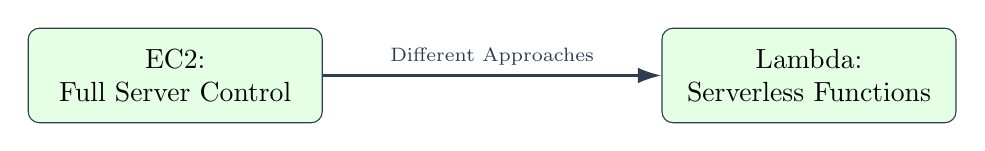
\begin{tikzpicture}[node distance=4.3cm]
            \node[serviceBox, fill=green!10, text width=3.5cm] (ec2) {EC2:\\Full Server Control};
            \node[serviceBox, fill=green!10, text width=3.5cm, right=4.3cm of ec2] (lambda) {Lambda:\\Serverless Functions};

            \draw[arrowLine] (ec2) -- node[above]{\scriptsize Different Approaches} (lambda);
        \end{tikzpicture}
    }
\end{center}
\textbf{EC2} is a virtual machine you configure. \textbf{Lambda} runs your code in response to events without you managing servers.

\subsection{Databases: RDS vs. DynamoDB}
\begin{center}
    \resizebox{0.85\textwidth}{!}{%
        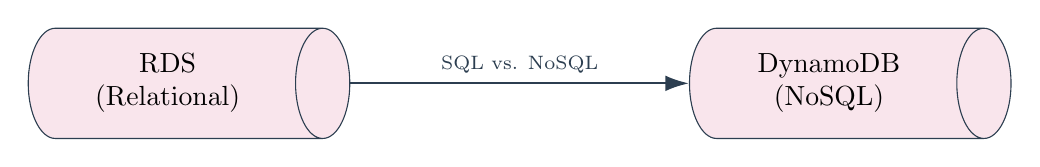
\begin{tikzpicture}[node distance=4.3cm]
            \node[database, fill=purple!10, text width=3cm] (rds) {RDS\\(Relational)};
            \node[database, fill=purple!10, text width=3cm, right=4.3cm of rds] (ddb) {DynamoDB\\(NoSQL)};

            \draw[arrowLine] (rds) -- node[above]{\scriptsize SQL vs. NoSQL} (ddb);
        \end{tikzpicture}
    }
\end{center}
\textbf{RDS} supports databases like MySQL or PostgreSQL, while \textbf{DynamoDB} is a key-value NoSQL store.

\subsection{CloudFront (CDN)}
Provides faster delivery of static or dynamic content by using "edge locations" near users around the world.

\subsection{Sample Lambda Code}
\begin{minted}[fontsize=\small, frame=single]{python}
def processImage(event, context):
    fileKey = event["Records"][0]["s3"]["object"]["key"]
    # Perform some image processing...
    return {"statusCode": 200, "body": "Success"}
\end{minted}

\clearpage

% --------------------------------------------------------
% 6. HANDS-ON PROJECT IDEAS
% --------------------------------------------------------
\section{Hands-On Project Ideas}
\justifying

\subsection{Beginner Projects}
\textbf{1. Static Website on S3/CloudFront}\\
Host a personal or portfolio site on S3, then speed it up globally with CloudFront.

\textbf{2. Simple File Processor}\\
When you upload a file, Lambda resizes or converts it. Great for learning event-driven tasks.

\subsection{Intermediate Projects}
\textbf{1. Full Web App (EC2, RDS, S3)}\\
Run a web server on EC2, store user data in RDS, and keep images in S3.

\textbf{2. Serverless API (API Gateway + Lambda + DynamoDB)}\\
Everything is serverless. Lambda handles business logic, DynamoDB stores data.

\subsection{Advanced Projects}
\textbf{1. Real-Time Data (Kinesis + Lambda + DynamoDB)}\\
Stream logs or sensor data into Kinesis, process in Lambda, save in DynamoDB.

\textbf{2. Machine Learning (SageMaker + S3 + Lambda)}\\
Store training data in S3, train a model with SageMaker, then call it via Lambda.

\begin{center}
    \resizebox{0.95\textwidth}{!}{%
        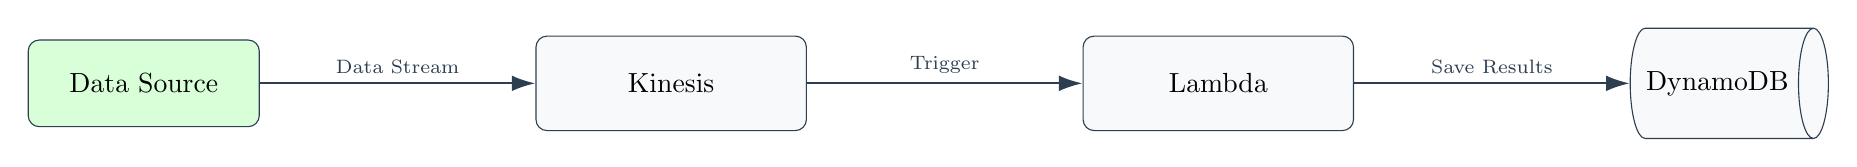
\begin{tikzpicture}[node distance=3.5cm]
            \node[userFigure] (source) {Data Source};
            \node[serviceBox, right=3.5cm of source] (kinesis) {Kinesis};
            \node[serviceBox, right=3.5cm of kinesis] (lambda) {Lambda};
            \node[database, right=3.5cm of lambda] (ddb) {DynamoDB};

            \draw[arrowLine] (source) -- node[above]{\scriptsize Data Stream} (kinesis);
            \draw[arrowLine] (kinesis) -- node[above]{\scriptsize Trigger} (lambda);
            \draw[arrowLine] (lambda) -- node[above]{\scriptsize Save Results} (ddb);
        \end{tikzpicture}
    }
\end{center}

\clearpage

% --------------------------------------------------------
% 7. EXTRA VISUALS & STEP-BY-STEP FLOWS
% --------------------------------------------------------
\section{Extra Visuals \& Step-by-Step Flows}
\justifying

\subsection{Typical User Request Flow}
\begin{center}
    \resizebox{0.95\textwidth}{!}{%
        \begin{tikzpicture}[node distance=3cm]
            \node[userFigure, text width=2.7cm] (user) {Client/User};
            \node[serviceBox, right=3.5cm of user, text width=3.2cm] (dns) {DNS Lookup};
            \node[serviceBox, right=3.5cm of dns, text width=3.2cm] (cloudfront) {CloudFront};
            \node[serviceBox, right=3.5cm of cloudfront, text width=3.2cm] (app) {App Layer (EC2/Lambda)};
            \node[database, right=3.5cm of app, text width=3.2cm] (db) {DB (RDS/DynamoDB)};

            \draw[arrowLine] (user) -- node[above]{\scriptsize 1. Request domain} (dns);
            \draw[arrowLine] (dns) -- node[above]{\scriptsize 2. Return IP} (cloudfront);
            \draw[arrowLine] (cloudfront) -- node[above]{\scriptsize 3. Forward Request} (app);
            \draw[arrowLine] (app) -- node[above]{\scriptsize 4. DB read/write} (db);
        \end{tikzpicture}
    }
\end{center}

\subsection{Simple Auto Scaling}
\begin{center}
    \resizebox{0.9\textwidth}{!}{%
        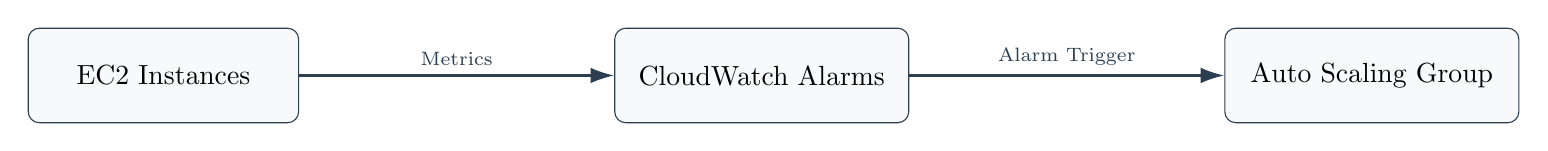
\begin{tikzpicture}[node distance=3.5cm]
            \node[serviceBox, text width=3.2cm] (ec2) {EC2 Instances};
            \node[serviceBox, text width=3.5cm, right=4cm of ec2] (cw) {CloudWatch Alarms};
            \node[serviceBox, text width=3.5cm, right=4cm of cw] (asg) {Auto Scaling Group};

            \draw[arrowLine] (ec2) -- node[above]{\scriptsize Metrics} (cw);
            \draw[arrowLine] (cw) -- node[above]{\scriptsize Alarm Trigger} (asg);
        \end{tikzpicture}
    }
\end{center}

\clearpage

% --------------------------------------------------------
% 8. A LEARNING PATH
% --------------------------------------------------------
\section{A Learning Path}
\justifying

\subsection{Step 1: Core Services}
\begin{itemize}
    \item \textbf{S3} for storing files
    \item \textbf{Lambda} for event-driven code
    \item \textbf{DynamoDB} for simple NoSQL
\end{itemize}

\subsection{Step 2: Building APIs and Servers}
\begin{itemize}
    \item \textbf{API Gateway} for REST calls
    \item \textbf{EC2} for custom servers
    \item \textbf{RDS} for relational data
\end{itemize}

\subsection{Step 3: Advanced Tools}
\begin{itemize}
    \item \textbf{Kinesis} for streaming data
    \item \textbf{SageMaker} for machine learning
    \item \textbf{Athena/Redshift} for analytics
\end{itemize}

\begin{center}
    \resizebox{0.9\textwidth}{!}{%
        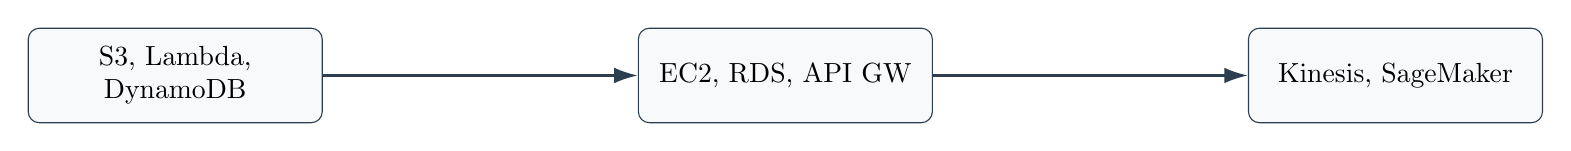
\begin{tikzpicture}[node distance=3cm]
            \node[serviceBox, text width=3.5cm] (basic) {S3, Lambda, DynamoDB};
            \node[serviceBox, right=4cm of basic, text width=3.5cm] (inter) {EC2, RDS, API GW};
            \node[serviceBox, right=4cm of inter, text width=3.5cm] (advanced) {Kinesis, SageMaker};

            \draw[arrowLine] (basic) -- (inter);
            \draw[arrowLine] (inter) -- (advanced);
        \end{tikzpicture}
    }
\end{center}

\clearpage

% --------------------------------------------------------
% CONCLUSION
% --------------------------------------------------------
\section*{Conclusion}
\addcontentsline{toc}{section}{Conclusion}
\justifying

AWS lets you run applications in the cloud instead of managing your own hardware. You can store static files in \textbf{S3}, launch code on \textbf{Lambda}, or run a full server via \textbf{EC2}. Distributing apps across Regions and Availability Zones improves reliability.

\textbf{Key Takeaways}:
\begin{itemize}
    \item \textbf{Start small}: Try a static site on S3 or a simple file-processor with Lambda.
    \item \textbf{Add complexity}: Use RDS or DynamoDB to store data, and CloudFront to speed up content delivery.
    \item \textbf{Explore advanced features}: Handle real-time data (Kinesis) or train machine learning models (SageMaker).
\end{itemize}

For more details, check out the
\href{https://aws.amazon.com/documentation/}{\textbf{official AWS docs}},
and use the \textbf{AWS Free Tier} to learn without large costs.

\end{document}
